\documentclass{article}

\usepackage[utf8]{inputenc}

\usepackage[a4paper, total={6in, 10in}]{geometry}
\usepackage{amsmath}

\usepackage{graphicx}

\usepackage{subcaption}

\title{Assignment 2}
\author{Leroy Souz}
\date{19th October 2024}

\begin{document}

\maketitle

\section*{Question 1.1}
The data matrix will be:
$$
X = \begin{bmatrix}
    1 & 4 & 1 & 1 \\
    1 & 7 & 0 & 2 \\
    1 & 10 & 1 & 3 \\
    1 & 13 & 0 & 4 \\
\end{bmatrix}
$$

\section*{Question 1.2}
The y vector [16, 23, 36, 43] is in the same hyperplane as the data matrix,
thus the answer will be exact

\section*{Question 1.3}
In the normal equation, $\Phi^t\Phi$ is not invertible so we have to solve it
using pseudo-inverse. We can calculate the pseudo-inverse by first calculating
the SVD of $\Phi$. The SVD of $\Phi$ is given by $\Phi = U \Sigma V^t$. We can
then calculate the pseudo-inverse of $\Phi$ as $\Phi^+ = V \Sigma^+ U^t$ where
$\Sigma^+$ is calculated by taking the reciprocal of the non-zero elements of
$\Sigma$ and then taking the transpose of the resulting matrix. Finally, we can
calculate the weights as $w = \Phi^+ t$.

\noindent After doing these calculations, we get the following weights:
$$
\vec{w} = \begin{bmatrix}
    0 \\
    3 \\
    3 \\
    1
\end{bmatrix}
$$

\section*{Question 1.4}
The model shown by the person is not same as mine. This has happened because for
the data matrix, the matrix does not have a full rank as well as, is linearly
dependant thus there exists infinitely many exact solutions that satisfy the 4
datapoints.

\section*{Question 1.5}
The new weights obtained by adding these points to the data matrix are:
$$
\vec{w} = \begin{bmatrix}
    0.0385 \\
    2.9947 \\
    3.0828 \\
    1.0111
\end{bmatrix}
$$

\noindent Due to infinitely many solutions available, the chance to get the same weights
as the person is close to 0.

\section*{Question 1.6}
To remove a column to ensure a unique solution, the resulting matrix should have
a full rank or $\Phi^t\Phi$ should be invertible. This can be done by removing
any column other than the 3rd column.

\section*{Question 2.1}
The MMSE objective function is given by:
$$
J(w) = \frac{1}{2} \sum_{n=1}^{2} (y_i - \hat{y_i})^2
$$

\noindent The optimal solution $(w_0, w_1)$ = $(1, 1)$

\section*{Question 2.2}
The Lagrangian function is given by:
$$
L(w, \lambda) = J(w) + \lambda (||\vec{w}||^2 - C )
$$

\section*{Question 2.3}
We can find the Lagrangian multiplier and weights by first taking the derivative of:
$$
\mathcal{L}(\vec{w}, \lambda) = \frac{1}{2} \left[ (1 - w_0)^2 + (1 - w_1)^2 \right] + \lambda \left( w_0^2 + w_1^2 - C \right)
$$

We take this derivative with respect to $w_0$, $w_1$, and $\lambda$ and set them to 0 to get the following equations:
\begin{align*}
    \frac{\partial}{\partial w_0} \left[ \frac{1}{2} (1 - w_0)^2 \right] = -(1 - w_0) + 2 \lambda w_0\\
    \frac{\partial}{\partial w_1} \left[ \frac{1}{2} (1 - w_1)^2 \right] = -(1 - w_1) + 2 \lambda w_1\\
    \frac{\partial}{\partial \lambda} \left[ \lambda (w_0^2 + w_1^2 - C) \right] = w_0^2 + w_1^2 - C
\end{align*}

Setting these equal to 0, we get the following equations:
\begin{align*}
    w_0 = \frac{1}{1 + 2\lambda}\\
    w_1 = \frac{1}{1 + 2\lambda}\\
    w_0^2 + w_1^2 = C
\end{align*}

Substituting the values of $w_0$ and $w_1$ in the third equation, we get:
\begin{align*}
    \frac{1}{(1 + 2\lambda)^2} + \frac{1}{(1 + 2\lambda)^2} = C\\
    \frac{2}{(1 + 2\lambda)^2} = C\\
    \lambda = \frac{\sqrt{\frac{2}{C}}-1}{2}
\end{align*}

For C = 0.5,
\begin{align}
    \lambda = \frac{\sqrt{\frac{2}{0.5}}-1}{2} = 0.5\\
    w_0 = w_1 = \frac{1}{1 + 2*0.5} = 0.5
\end{align}

For C = 1,
\begin{align}
    \lambda = \frac{\sqrt{\frac{2}{1}}-1}{2} = 0.21\\
    w_0 = w_1 = \frac{1}{1 + 2*0} = 0.70
\end{align}

For C = 2,
\begin{align}
    \lambda = \frac{\sqrt{\frac{2}{2}}-1}{2} = 0\\
    w_0 = w_1 = \frac{1}{1 + 2*0} = 1
\end{align}

For C = 3,
\begin{align}
    \lambda = \frac{\sqrt{\frac{2}{3}}-1}{2} = 0\\
    w_0 = w_1 = \frac{1}{1 + 2*0} = 1
\end{align}



\section*{Question 3.1}
The average validation error across the 5 cv is: 0.6874

\section*{Question 3.2}
The best $\lambda$ found by me is: 0.0001.\\
The plot is shown below:\\
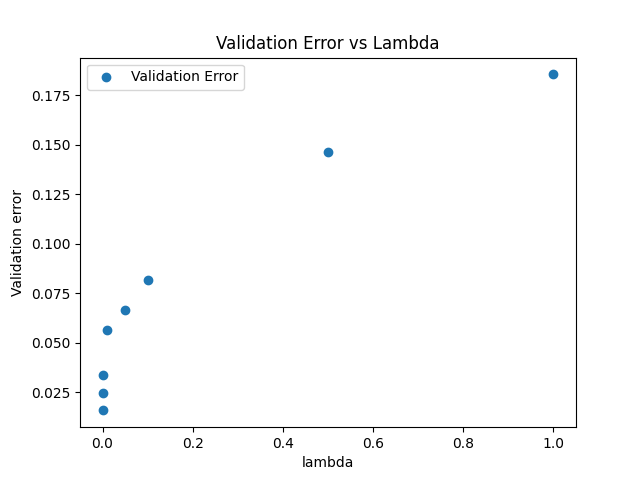
\includegraphics{/home/sprutz/dev/mlp/HW2/images/val_error_ridge.png}

\section*{Question 3.3}
Plot shown below:\\
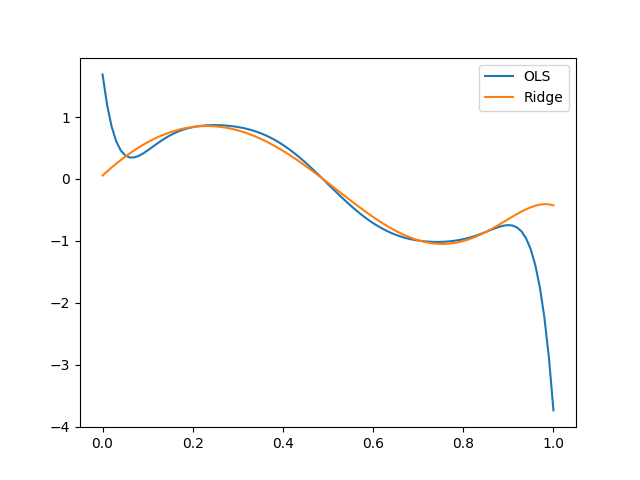
\includegraphics{/home/sprutz/dev/mlp/HW2/images/model_eval.png}

\section*{Question 3.4}
The MSE for ordinary MMSE is: 0.4439\\
The MSE for Ridge regression is: 0.0376

\section*{Question 3.5}
The plot for regression with more datapoints is shown below:\\
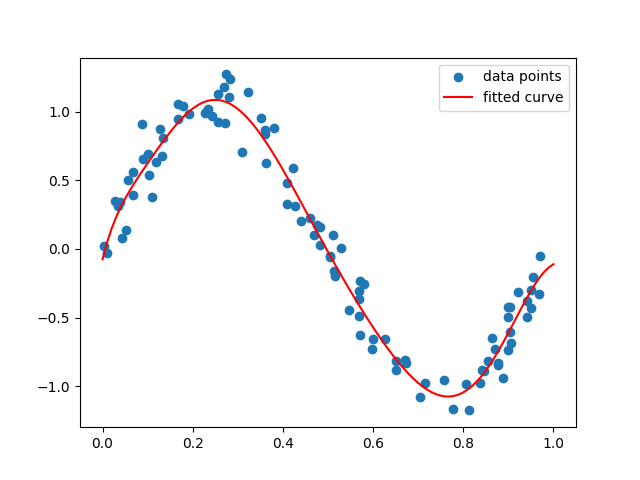
\includegraphics{/home/sprutz/dev/mlp/HW2/images/large_plot.png}

\section*{Question 3.6}
The two possible solutions to control model complexity are:\\
1. Increase the number of datapoints\\
2. Perform regularization

\section*{Question 4.1}
Calculated in q4.py

\section*{Question 4.2}
The 5 images are shown below:\\
\begin{figure}[h]
    \centering
    \begin{subfigure}[b]{0.18\textwidth}
        \centering
        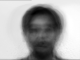
\includegraphics[width=\textwidth]{/home/sprutz/dev/mlp/HW2/images/reconst(M=2).png}
        \caption{M=2}
    \end{subfigure}
    \begin{subfigure}[b]{0.18\textwidth}
        \centering
        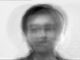
\includegraphics[width=\textwidth]{/home/sprutz/dev/mlp/HW2/images/reconst(M=10).png}
        \caption{M=10}
    \end{subfigure}
    \begin{subfigure}[b]{0.18\textwidth}
        \centering
        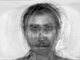
\includegraphics[width=\textwidth]{/home/sprutz/dev/mlp/HW2/images/reconst(M=100).png}
        \caption{M=100}
    \end{subfigure}
    \begin{subfigure}[b]{0.18\textwidth}
        \centering
        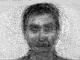
\includegraphics[width=\textwidth]{/home/sprutz/dev/mlp/HW2/images/reconst(M=1000).png}
        \caption{M=1000}
    \end{subfigure}
    \begin{subfigure}[b]{0.18\textwidth}
        \centering
        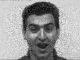
\includegraphics[width=\textwidth]{/home/sprutz/dev/mlp/HW2/images/reconst(M=4000).png}
        \caption{M=4000}
    \end{subfigure}
    \caption{Reconstruction results with varying M values}
\end{figure}

\section*{Question 4.3}
Represnting the eigenvectors as images, we get the following images:\\
\begin{figure}[h]
    \centering
    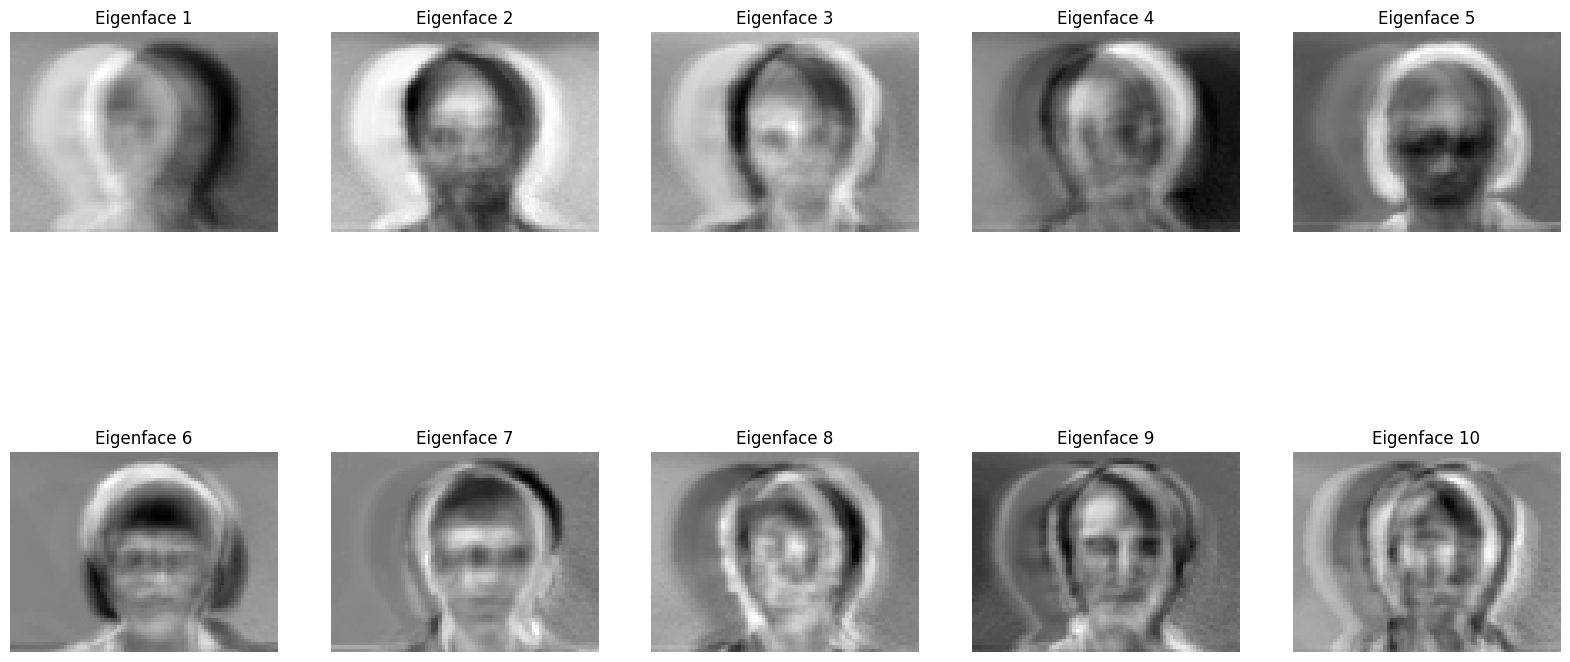
\includegraphics[width=0.8\textwidth]{/home/sprutz/dev/mlp/HW2/images/eigenfaces.png}
    \caption{Eigenfaces represented as images}
\end{figure}

\noindent Oberservations:
\begin{enumerate}
    \item \textbf{Eigenface 1}: Captures the most general features of the face, such as overall lighting and orientation. It emphasizes the general structure of a face (e.g., head shape and position).
    \item \textbf{Eigenface 2}: Focuses more on facial features like the eyes and nose. It may also capture some variations in lighting or pose.
    \item \textbf{Eigenface 3}: Highlights more detailed facial features, such as the contrast between the eyes, nose, and mouth regions.
    \item \textbf{Eigenface 4}: Captures finer details, possibly related to the positioning of the eyes and eyebrows, and some variations in the face's upper region.
    \item \textbf{Eigenface 5}: Focuses on variations in the middle and lower parts of the face, such as the mouth and chin area.
    \item \textbf{Eigenface 6}: Emphasizes variations in the hairline and forehead, as well as some details around the eyes.
    \item \textbf{Eigenface 7}: Captures subtle differences in the facial structure, particularly around the eyes and nose.
    \item \textbf{Eigenface 8}: Highlights variations in the face's overall shape, especially around the cheeks and jawline.
    \item \textbf{Eigenface 9}: Focuses on asymmetries in the face, such as differences between the left and right sides of the face.
    \item \textbf{Eigenface 10}: Captures very specific details, such as small variations in the eyes, nose, and mouth, and possibly some distortions or lighting variations.
\end{enumerate}

\newpage
\section*{Question 5.1}
The reproducted plots are shown below:\\
\begin{figure}[h]
    \centering
    \begin{subfigure}[b]{0.45\textwidth}
        \centering
        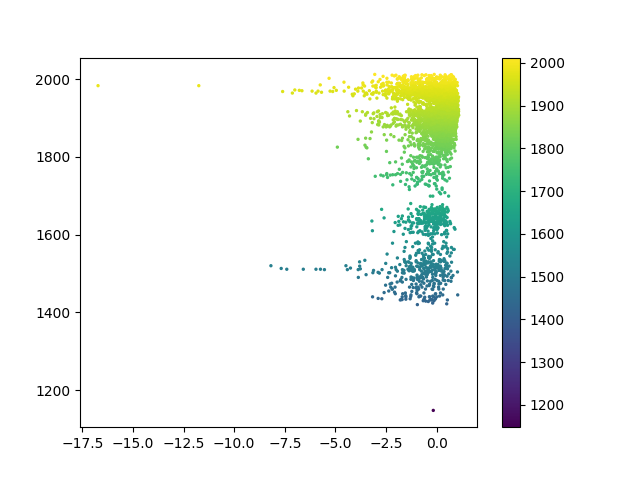
\includegraphics[width=\textwidth]{/home/sprutz/dev/mlp/HW2/images/2dplot.png}
        \caption{5.1.1}
    \end{subfigure}
    \begin{subfigure}[b]{0.45\textwidth}
        \centering
        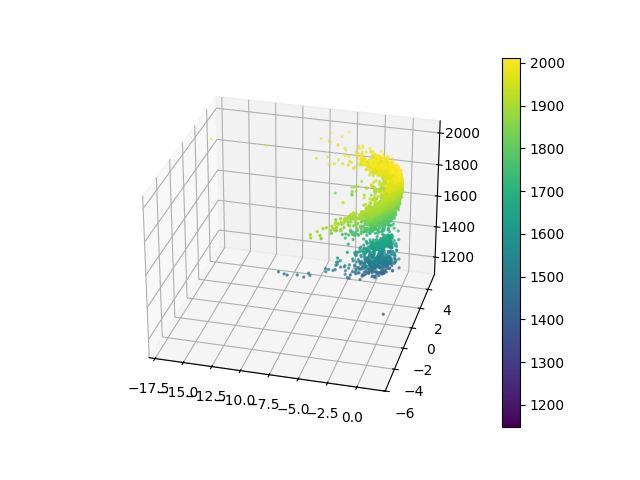
\includegraphics[width=\textwidth]{/home/sprutz/dev/mlp/HW2/images/3dplot.png}
        \caption{5.1.2}
    \end{subfigure}
    \caption{Reproducted plots}
\end{figure}

\noindent Based on the figures one can conclude that more variation will be captured in the
2d projection because it captures more variance and thus more information is available
for the model to predict the target variable.

\section*{Question 5.2}
The validation on MSE is 6509 with a good basis function being of degree 5.

\section*{Question 5.3}
The MSE on the test set is 6592

\noindent The most accurate prediction was on file '4304\_alfred-sisley-1876.jpg' being predicted as 1876.\\
The least accurate prediction was on file '847\_polyptych-of-st-luke-1455.jpg' being predicted as 1886.




\end{document}
